\subsection{One-pass Algorithms}
%{One-pass algorithms that enforce the local checking policy}.
%The local checking policy \eat{, the key to achieve the \emph{one-pass} processing,} does not need a window to buffer the preview read points.
%Instead, it processes each point in a trajectory once and only once. % when compressing the trajectory.
%Obviously, the one-pass algorithms have a linear time complexity.

One-pass algorithms adopt local checking policies, and run in $O(n)$ time with an $O(1)$ space complexity. They are typically designed for specific distance metrics.

Reumann-Witkam (\rwa) \cite{Reumann:Strip} is a straightforward one-pass algorithm that builds a strip paralleling to the line connecting the first two points, then the points within this strip compose a section of the line.  \rwa is fast, but has a poor compression ratio.
Algorithm \operb~\cite{Lin:Operb} recently improves \rwa  by allowing dynamically adjustable strips, together with several detailed optimization techniques.
%
There is also algorithm \siped (\emph{sector intersection}) that converts \ped distance tolerances into angle tolerances to speed up the process, which is {\em completely overlooked} by existing trajectory compression studies,  but can be easily adopted for trajectory compression, as it is originally developed in fields of computational geometry and pattern recognition~\cite{Williams:Longest,Sklansky:Cone,Dunham:Cone, Zhao:Sleeve}.
\eat{
	Initially, Williams~\cite{Williams:Longest} and Sklansky and Gonzalez \cite{Sklansky:Cone} proposed linear time algorithms based on the idea of ``cone intersection" in a plane, then Dunham \cite{Dunham:Cone} extended these algorithms, and the Sleeve algorithm \cite{Zhao:Sleeve} in the cartographic discipline essentially applied the same idea as \siped but alternatively called it ``sector intersection".
}%
These algorithms are dedicatedly designed  for \ped. {\em Algorithms \operb and \siped have good compression ratios, and, hence, we choose them as the representatives of  one-pass algorithms using \ped}.


Algorithm Linear Dead Reckoning (\ldr) for position tracking \cite{Trajcevski:DDR} follows the similar routine as \rwa except that it uses and assumes a velocity ${\vv{v}}$ for each section. \textcolor{blue}{\cite{Trajcevski:DDR} proves that if \ldr uses $\epsilon/2$ as the threshold in position tracking, then its output trajectory has a max error not greater than $\epsilon$ to the original trajectory. Thus, it can be treated as a trajectory simplification algorithm as well.}
It has poor compression ratios because both the value and the direction of velocity ${\vv{v}}$ are pre-defined and fixed between two updates, \myblue{and it indeed uses a half $\epsilon$}.
Recently algorithm \cised~\cite{Lin:Cised} extends the \textit{sector intersection} method \siped from a 2D space to a spatio-temporal 3D space.
These one-pass algorithms are dedicatedly designed for \sed. {\em As algorithm \cised has a compression ratio close to algorithm \dpa using \sed, we choose it as the representative of one-pass algorithms using \sed}.


{Direction range intersection} approaches are similar to  \emph{sector intersection} methods except that they are designed for \dad, and {\em we choose \intersec \cite{Long:Direction} and \interval \cite{Ke:Interval} as the representatives of one-pass algorithms using \dad}.

\textcolor{blue}{Algorithms \siped, \ldr, \operb, \cised and \intersec share a common idea, \ie using a half-$\epsilon$ to implement the strong simplification to ensure that the max error does not exceed $\epsilon$. In the sequel, we shall discuss that the half-$\epsilon$ of \siped and \cised can be extended to the full-$\epsilon$ with some small modifications, along the similar way that \interval extends \intersec. }

\eat{%%%%%%%%%%%%%%%%%%%%%%%%%%%%%%%%%%%%%%%%%%%%%%%%%%%%%%%
	
	The $n^{th}$ point routine and the routine of random-selection of points \cite{Shi:Survey} are two naive one-pass algorithms.
	In these routines, for every fixed number of consecutive points along the line, the $n^{th}$ point and one random point among them are retained, respectively.
	They run fast, however, they are not error bounded.
	
	\subsubsection{Reumann-Witkam and LDR}
	
	\begin{figure*}[tb!]
		\centering
		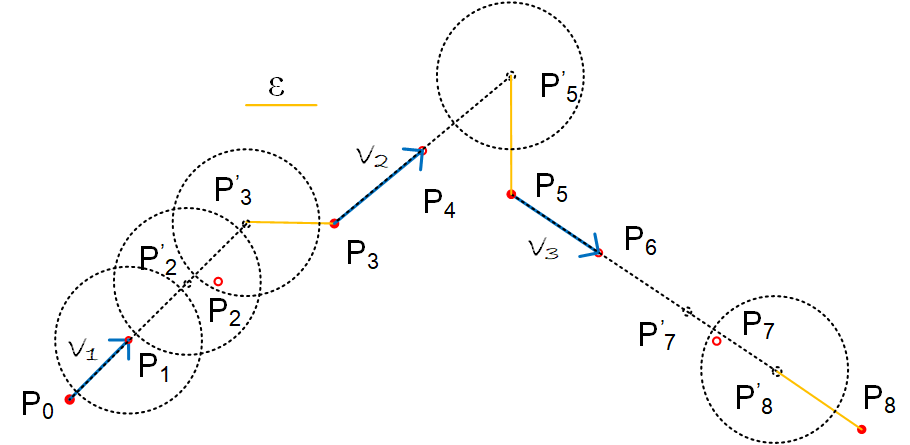
\includegraphics[scale=0.66]{Figures/Fig-LDR.jpg}
		\vspace{-1ex}
		\caption{\small The trajectory $\dddot{\mathcal{T}}[P_0, \ldots, P_{10}]$ is compressed by the Reumann-Witkam and Linear Dead Reckoning algorithms to four and eight line segments, respectively.}
		\vspace{-2ex}
		\label{fig:ldr}
	\end{figure*}
	
	In Reumann-Witkam\cite{Reumann:Strip}, the input data is divided into sections by strips.
	Initially, the first strip, with the width of $2*\epsilon$, takes the line $\vv{P_0P_1}$ connecting the first two points, $P_0$ and $P_1$ as its middle line.
	Then the strip is expending over the line into the direction of its initial tangent, covering the succeed points, $P_2, \ldots, P_{j}$, until the strip hits the line $\vv{P_jP_{j+1}}$ (meaning that the next point $P_{j+1}$, $j>1$, is out side of the strip).
	The points, $[P_0, \ldots, P_{j}]$, within this strip compose a section. The first and last points of the section, \ie $P_0,P_{j}$, are output, and those points between them are removed.
	The last point $P_{j}$ is the initial point of the next strip.
	The whole process is repeated until the strip contains the end point $P_n$ of the input data.
	The Reumann-Witkam is a one-pass algorithm.
	
	{The Linear Dead Reckoning (LDR)\cite{Lange:Tracking} for position tracking follows the similar routine as the Reumann-Witkam algorithm except that it assumes a velocity ${\vv{v}}$ for each section and uses \sed instead of \ped in distance checking.
		Moreover, the authors of \cite{Trajcevski:DDR} proved that LDR is also suitable for online spatio-temporal compression as long as the tolerance threshold of the algorithm is set to $\epsilon/2$.}
	
	\begin{example}
		\label{exm-alg-strip}
		In Figure~\ref{fig:ldr}, the trajectory $\dddot{\mathcal{T}}[P_0, \ldots, P_{10}]$ is compressed
		%
		(1) by the Reumann-Witkam to four line segments $\vv{P_0P_2}$, $\vv{P_2P_4}$, $\vv{P_4P_7}$ and $\vv{P_7P_{10}}$. First, a strip with width $2\epsilon$ is built parallel to the line $\vv{P_0P_1}$, then the strip is extended over the line and includes point $P_2$. Because $P_3$ is outside of the strip, $P_2$ becomes the end point of the first section and the start point of the second section.
		%
		(2) by the Linear Dead Reckoning algorithm to eight line segments $\vv{P_0P_1}$, $\vv{P_1P_2}$, $\vv{P_2P_3}$, $\vv{P_3P_4}$, $\vv{P_4P_5}$, $\vv{P_5P_7}$, $\vv{P_7P_8}$ and $\vv{P_8P_{10}}$. First, an initial velocity ${\vv{v}_0}$ is set to $|P_0P_1|/(t_1-t_0)$. Then the synchronized point $P'_2$ of $P_2$ is estimated based on the velocity ${\vv{v}_0}$ and time of $P_2$, \ie ${v}_0 * (t_2-t_0)$. Because the \sed from $P_2$ to the line $\vv{P_0P'_2}$ , \ie $|P_2P'_2|$, is great than $\epsilon/2$, the algorithm outputs $\vv{P_0P_1}$ and starts the next section.
	\end{example}
	
}%%%%%%%%%%%%%%%%%%%%%%%%%%%%%%%%%%%%%%%%%%%%%%%%%%%%%%%End of Eat


\subsubsection{{Algorithm \operb Using \ped} \cite{Lin:Operb}}
It designs a local distance checking method to dynamically adjust the direction of line segments to achieve an effective one-pass process. \textcolor{blue}{It has strong and weak versions, called \operb and \operb-A, respectively. \operb-A shares the same routine as \operb except that it applies a lazy output policy and allows data interpolations.}

Consider an error bound $\epsilon$ and a sub-trajectory $\dddot{\mathcal{T}_s}[P_s,$ $\ldots, P_{s+k}]$.
\operb dynamically maintains a directed line segment $\mathcal{L}_i$ ($i\in[1,k]$), whose start point is fixed with $P_s$ and its end point is identified (may not in $\{P_s, \ldots, P_{s+i}\}$) to {\em fit} all the previously processed points $\{P_s, \ldots, P_{s+i}\}$.
The directed line segment $\mathcal{L}_i$ is built by a function named \emph{fitting function $\mathbb{F}$}, such that when a new point $P_{s+i+1}$ is considered, only its distance to the directed line segment $\mathcal{L}_i$ is checked, instead of checking the distances of all or a subset of data points of $\{P_{s}, \ldots, P_{s+i}\}$ to $\mathcal{R}_{i+1}$ = $\vv{P_sP_{s+i+1}}$ as the global distance checking does.
During processing, if the distance of point $P_{s+i}$ to the directed line segment $\mathcal{L}_{i-1}$ is larger than the threshold, then a directed line segment, start from $P_s$, is generated and output;
otherwise, the directed line segment $\mathcal{L}_i$ is updated by the fitting function $\mathbb{F}$, as follows.

\begin{small}
	\vspace{-1ex}
	\begin{equation*}
	\label{equ-function}
	\left\{
	\hspace{1ex}\begin{aligned}
	&\left[
	\begin{aligned}
	% & |\mathcal{L}_{i}| = |\mathcal{R}_{i-1}|    \\
	% & \mathcal{L}_{i}.\theta = \mathcal{R}_{i-1}.\theta\\
	& \mathcal{L}_{i} = \mathcal{L}_{i-1}\\
	\end{aligned}
	\right]\hspace{12.5ex}~when~(|\mathcal{R}_{i}| - |\mathcal{L}_{i-1}|) \le \frac{\epsilon}{4}   \\
	&\hspace{-1.5ex}\left[
	\begin{aligned}
	& |\mathcal{L}_{i}|  = j*{\epsilon}/{2} \\
	& \mathcal{L}_{i}.\theta = \mathcal{R}_{i}.\theta    \\
	\end{aligned}
	\right]\hspace{8.5ex}~when~|\mathcal{R}_{i}| >  \frac{\epsilon}{4}~\And~|\mathcal{L}_{i-1}|=0    \\
	&\hspace{-1.5ex}\left[
	\begin{aligned}
	& |\mathcal{L}_{i}|  = j*{\epsilon}/{2}\\
	& \mathcal{L}_{i}.\theta = \mathcal{L}_{i-1}.\theta + f(\mathcal{R}_i,\mathcal{L}_{i-1})*\arcsin(\frac{ped(P_{s+i}, \mathcal{L}_{i-1})}{j*\epsilon/2})/j \\	
	% & \theta^- = \mathcal{L}_{i-1}.\theta - \arcsin(\frac{d(P_i, \mathcal{L}_{i-1})}{j*\epsilon/2})/j \\	
	% & \mathcal{L}_{i}.\theta = \arg_{\mathcal{L}_{i}.\theta}\min({d(P_{i+1}, \mathcal{L}_{i}}), \mathcal{L}_{i}.\theta \in\{\theta^+,\theta^-\})\\	
	\end{aligned}
	\right]\hspace{0ex}else\\
	\end{aligned}
	\right.
	\end{equation*}
	\vspace{0ex}
\end{small}


\ni where (a) $1 \le i \le k+1$; (b) $\mathcal{R}_{i-1}$ = $\vv{P_sP_{s+i-1}}$, is the directed line segment whose end point $P_{s+i-1}$ is in $\dddot{\mathcal{T}_s}[P_s, \ldots, P_{s+k}]$; (c) $\mathcal{L}_{i}$ is the directed line segment built by fitting function $\mathbb{F}$ to fit sub-trajectory $\dddot{\mathcal{T}_s}[P_s, \ldots, P_{s+i}]$ and $\mathcal{L}_{0}$ = $\mathcal{R}_{0}$; (d) $j = \lceil(|\mathcal{R}_{i}|*2/\epsilon - 0.5)\rceil$; (e) $f()$ is a sign function such that $ f(\mathcal{R}_i,\mathcal{L}_{i-1})$ = $1$ if the included angle $\angle(\mathcal{R}_{i-1}, \mathcal{R}_{i})$ = $(\mathcal{R}_i.\theta - \mathcal{L}_{i-1}.\theta)$ falls in the range of $(-2\pi, -\frac{3\pi}{2}]$, $[-\pi, -\frac{\pi}{2}]$, $[0, \frac{\pi}{2}]$ and $[\pi, \frac{3\pi}{2})$, and $f(\mathcal{R}_i,\mathcal{L}_{i-1})$ = $-1$, otherwise; (f) $\epsilon/2$ is a step length to control the increment of $|\mathcal{L}|$.
%
Optimizations are developed to achieve better compression ratios.


\begin{example}
	\label{exm-alg-operb}
	Figure~\ref{fig:operb} is a running example of the \operb algorithm compressing the same trajectory $\dddot{\mathcal{T}}[P_0, \ldots, P_{10}]$.
	(1) It takes $P_0$ as the start point, reads $P_1$ and sets $\mathcal{L}_1$ = $\vv{P_0P_1}$.
	(2) It reads $P_2$. The distance from $P_2$ to $\mathcal{L}_1$ is less than the threshold, thus, it updates $\mathcal{L}_1$  to $\mathcal{L}_2$ by the fitting function $\mathbb{F}$.
	(3) It reads $P_3$ and $P_4$, and updates $\mathcal{L}_2$ to $\mathcal{L}_3$ and $\mathcal{L}_3$ to $\mathcal{L}_4$, respectively.
	(4) It reads $P_5$. The distance from $P_5$ to $\mathcal{L}_4$ is larger than the threshold, thus, it outputs $\vv{P_0P_4}$ and starts the next section taking $P_4$ as the new start point.
	(5) The process continues until all points have been processed. At last, the algorithm outputs two continuous line segments $\vv{P_0P_4}$ and $\vv{P_4P_{10}}$.
\end{example}


\begin{figure}[tb!]
	\centering
	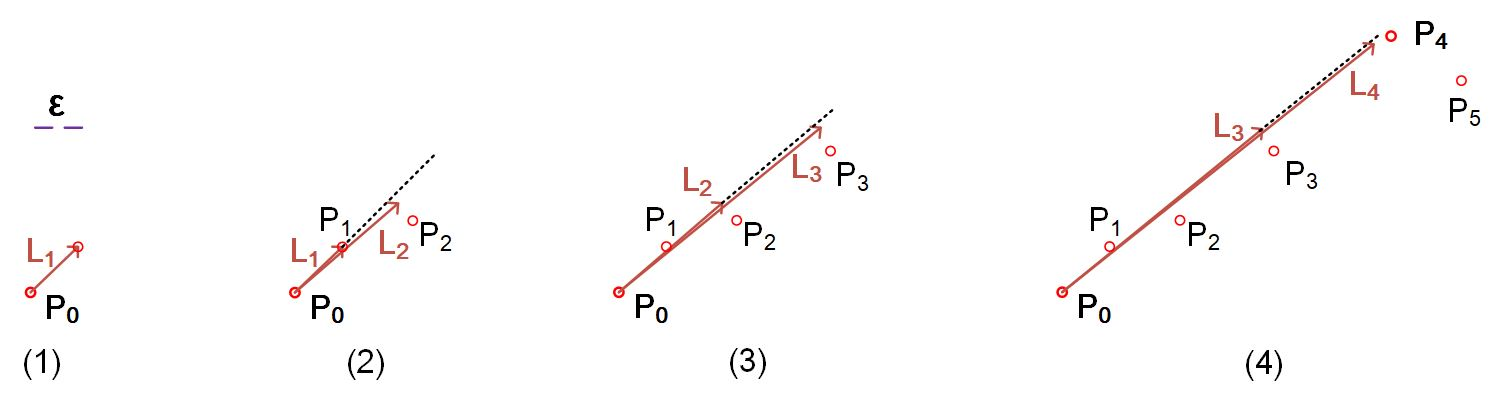
\includegraphics[scale=0.66]{Figures/Fig-OPER.jpg}
	\vspace{-1ex}
	\caption{\small The trajectory $\dddot{\mathcal{T}}[P_0, \ldots, P_{10}]$ is compressed by the \operb algorithm using \ped to two line segments.}
	\vspace{-1ex}
	\label{fig:operb}
\end{figure}


\subsubsection{Algorithm \siped Using \ped \cite{Williams:Longest, Sklansky:Cone, Dunham:Cone, Zhao:Sleeve}}
It develops a concept of ``Sector'' \cite{Williams:Longest, Sklansky:Cone, Dunham:Cone, Zhao:Sleeve}, which converts the distance tolerance into an angle change tolerance for checking  points.

Given a sequence of points $[P_{s}, P_{s+1}, \ldots, P_{s+k}]$ and an error bound $\epsilon$,
for the start data point $P_s$, any point $P_{s+i}$ and $|\vv{P_sP_{s+i}}|>\epsilon$ ($i\in[1, k]$), there are two directed lines $\vv{P_sP^u_{s+i}}$ and $\vv{P_sP^l_{s+i}}$ such that $ped(P_{s+i}, \vv{P_sP^u_{s+i}})$ $=$ $ped(P_{s+i}, \vv{P_sP^l_{s+i}}) = \epsilon$ and either ($\vv{P_sP^l_{s+i}}.\theta < \vv{P_sP^u_{s+i}}.\theta ~and~\vv{P_sP^u_{s+i}}.\theta - \vv{P_sP^l_{s+i}}.\theta <\pi$) or ($\vv{P_sP^l_{s+i}}.\theta > \vv{P_sP^u_{s+i}}.\theta ~and~ \vv{P_sP^u_{s+i}}.\theta - \vv{P_sP^l_{s+i}}.\theta < -\pi)$. Indeed, they form a \emph{sector} \sector{(P_s, P_{s+i}, \epsilon)} that takes $P_s$ as the center point and $\vv{P_sP^u_{s+i}}$ and $\vv{P_sP^l_{s+i}}$ as the borderlines.
%
There exists a data point $Q$ such that for any data point $P_{s+i}$ ($i \in [1, ... k]$), its perpendicular Euclidean distance to
directed line $\overline{P_sQ}$ is not greater than the error bound $\epsilon$ if and only if the $k$ sectors \sector{(P_s, P_{s+i}, \epsilon)} ($i\in[1,k]$) share common data points other than $P_s$, \ie $\bigsqcap_{i=1}^{k}$\sector{(P_s, P_{s+i}, \epsilon)} $\ne \{P_s\}$ \cite{Williams:Longest, Sklansky:Cone,Zhao:Sleeve}.
%
Here, point $Q$ may not belong to $\{P_{s}, P_{s+1},$ $\ldots, P_{s+k}\}$.
However, if $Q$ must be a point selected from the original points, in other words, point $P_{s+i}$ ($1\le i\le k$) is chosen as $Q$, then
for any point $P_{s+j}$ ($j \in [1, ... i]$), its \ped to
line segment $\overline{P_sP_{s+i}}$ is not greater than the error bound $\epsilon$ if $\bigsqcap_{j=1}^{i}$\sector{(P_s, P_{s+j}, \epsilon/2)} $\ne \{P_s\}$, as pointed out in \cite{Zhao:Sleeve}.
That is, {\em these sector intersection based algorithms can be easily adopted for trajectory compression}.
In practice, it is a good choice to set the point $Q$ as the point among all points in $[P_{s}, P_{s+1}, \ldots, P_{s+k}]$ that has the longest distance to $P_s$.


The original \siped uses a half sector, $\frac{\epsilon}{2}$-\sector, which may limit its compression performance. However, it can further be extended to a full ${\epsilon}$-\sector ~ by adding a constraint. That is, for any point $P_{s+j}$ ($j \in [1, ... i]$), its \ped to
line segment $\overline{P_sP_{s+i}}$ is not greater than the error bound $\epsilon$ if $ P_{s+i} \ne {P_s}$ and $P_{s+i}\in \bigsqcap_{j=1}^{i-1}$\sector{(P_s, P_{s+j}, \epsilon)}, \ie $P_{s+i}$ lives in the common intersection of preview full \emph{sectors}.



\begin{example}
	\label{exm-alg-sleeve}
	Figure~\ref{fig:sleeve} is a running example of algorithm \siped($\frac{\epsilon}{2}$) taking as input the same trajectory $\dddot{\mathcal{T}}[P_0, \ldots, P_{10}]$. At the beginning, $P_0$ is the first start point, and points $P_1$, $P_2$, $P_3$, etc., each has a narrow \emph{sector}.
	For example, the narrow \emph{sector} $\mathcal{S}$($P_0$, $P_{3}$, $\epsilon/2$) takes $P_0$ as the center point and $\vv{P_0P^u_{3}}$ and $\vv{P_0P^l_{3}}$ as the borderlines.
	Because $\bigsqcap_{i=1}^{4}\mathcal{S}(P_0, P_{0+i}, \epsilon/2) \ne \{P_0\}$ and $\bigsqcap_{i=1}^{5}\mathcal{S}(P_0, P_{0+i}, \epsilon/2) = \{P_0\}$, $\vv{P_0P_4}$ is output and $P_4$ becomes the start point of the next section.
	At last, the algorithm outputs two continuous line segments $\vv{P_0P_4}$ and $\vv{P_4P_{10}}$.
\end{example}

\begin{figure}[tb!]
	\centering
	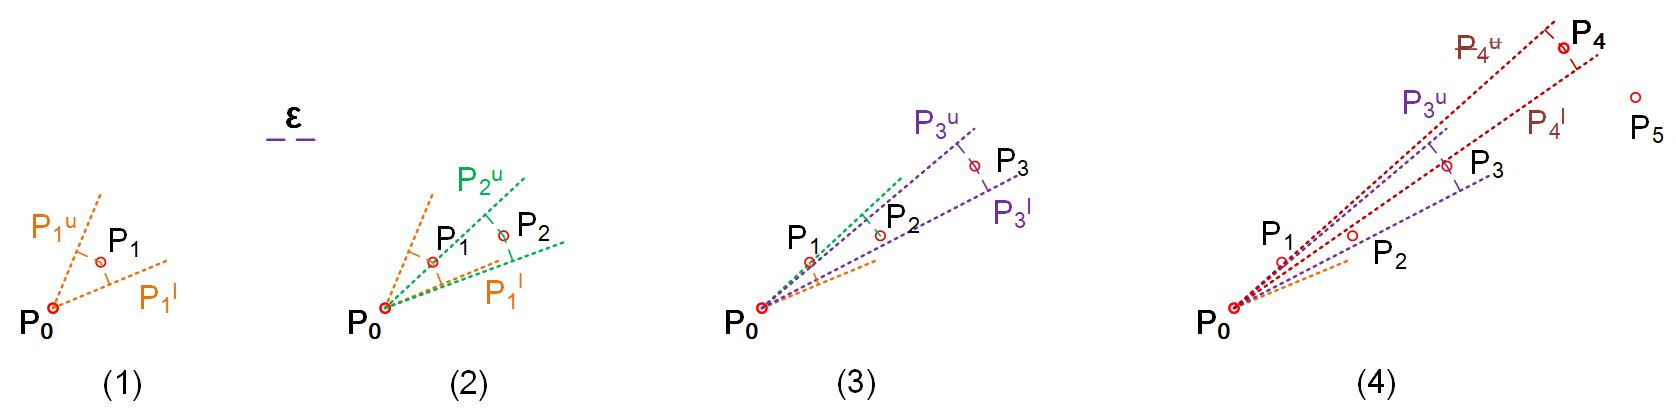
\includegraphics[scale=0.66]{Figures/Fig-sleeve.jpg}
	\vspace{-2ex}
	\caption{\small The trajectory $\dddot{\mathcal{T}}$ is compressed by the sector intersection algorithm using \ped to two line segments.}
	\vspace{-1ex}
	\label{fig:sleeve}
\end{figure}




\subsubsection{Algorithm \cised Using \sed \cite{Lin:Cised}}
It develops an idea of \textit{spatio-temporal cone} that extends the \textit{sector intersection} method \cite{Williams:Longest, Sklansky:Cone, Dunham:Cone, Zhao:Sleeve} from an \textcolor{blue}{\em x-y} 2D space to an \textcolor{blue}{\em x-y-t} spatio-temporal 3D space.
\textcolor{blue}{Note that for computer graphics and cartography, there is another 3D space, \ie \emph{x-y-z} 3D space, where {\em z} is the height. There are studies \cite{Barequet:3D, Eu:Ln3D} for solving the \emph{min-\#} and \emph{min-$\epsilon$} problems in the \emph{x-y-z} 3D space, \eg \cite{Barequet:3D} extends the \textit{sector intersection} method to the \textit{off-line ball-inclusion testing} in the \emph{x-y-z} 3D space, so as to develop efficient near quadratic time algorithms.} %

Given a sub-trajectory $[P_s,...,P_{s+k}]$ and an error bound $\epsilon$, any point $P'_{s+i}$ ($0< i \le k$) on the plane $P.t-P_{s+i}.t = 0$ is a synchronized data point of $P_{s+i}$. For all $P'_{s+i}$ in the plane satisfying $|P_{s+i}P'_{s+i}| \le \epsilon$, they form a \textit{synchronous circle $\mathcal{O}(P_{s+i}, \epsilon)$} of $P_{s+i}$ with $P_{s+i}$ as its center and $\epsilon$ as its radius.
%
A spatio-temporal cone (or simply \textit{cone}) of a data point $P_{s+i}$ ($1\le i\le k$) in $\dddot{\mathcal{T}}_s$ \wrt a point $P_s$ and an error bound $\epsilon$, denoted as \cone{(P_s, \mathcal{O}(P_{s+i}, \epsilon))}, or \cone{_{s+i}} in short, is an oblique circular cone such that point $P_s$ is its apex and the synchronous circle $\mathcal{O}(P_{s+i}, \epsilon)$ is its base.
%
Then, there exists a point $Q$ such that $Q.t = P_{s+k}.t$ and $sed(P_{s+i}, \vv{P_sQ})\le \epsilon$ for each $i \in [1,k]$ if and only if $\bigsqcap_{i=1}^{k}$\cone{(P_s, \mathcal{O}(P_{s+i}, \epsilon))} $\ne \{P_s\}$.
%
Like \textit{sector intersection} methods, point $Q$ may also not belong to $\{P_{s}, P_{s+1},$ $\ldots, P_{s+k}\}$.
\textcolor{blue}{If point $Q$ is not necessarily in  $\{P_{s}, P_{s+1},$ $\ldots, P_{s+k}\}$, then this algorithm is a weak simplification, named \cised-W that uses a full-$\epsilon$ cone.}
If point $Q$ must be $P_{s+i}$ ($1\le i\le k$), then for any point $P_{s+j}$ ($j \in [1, ... i]$), its \sed to line segment $\overline{P_sP_{s+i}}$ is not greater than the error bound $\epsilon$ if
$\bigsqcap_{j=1}^{i}$\cone{(P_s, P_{s+j}, \epsilon/2)} $\ne \{P_s\}$ as pointed out in \cite{Lin:Cised}.
\textcolor{blue}{This algorithm, named \cised($\frac{\epsilon}{2}$) that uses a half-$\epsilon$ cone, belongs to strong simplification.}
\textcolor{blue}{Moreover, \cised($\frac{\epsilon}{2}$) can also be extended to \cised(${\epsilon}$), another strong version that uses a full-${\epsilon}$ cone,} by adding a constraint that $P_{s+i}$ lives in the common intersection of preview full \emph{cones}.

In addition, because these spatio-temporal cones have the same apex $P_s$, the checking of their intersection can be computed by a much simpler way, \ie the checking of the intersection of cone projection circles on a plane, and a circle is further approximated with its $m$-edge inscribed regular polygon, whose intersection can be computed more efficiently. %



\eat{
	\begin{figure}[tb!]
		\centering
		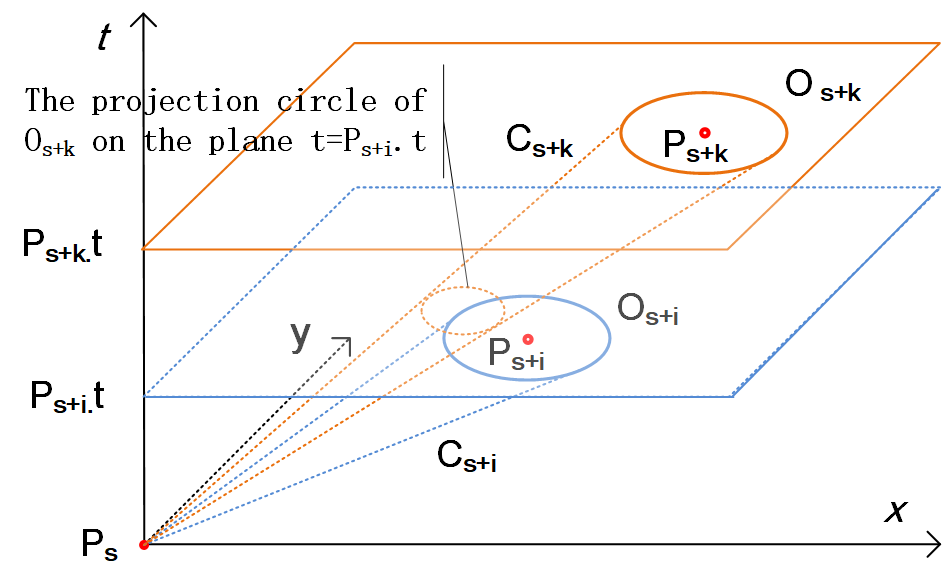
\includegraphics[scale=0.66]{Figures/Fig-CIS.jpg}
		\vspace{-3ex}
		\caption{\small Examples of spatio-temporal cones.} % in a 3D Cartesian coordinate system
		\vspace{-2ex}
		\label{fig:cis}
	\end{figure}
}


%%%%%%%%%%%%%%% example of Algorithm CISED
\begin{figure}[tb!]
	\centering
	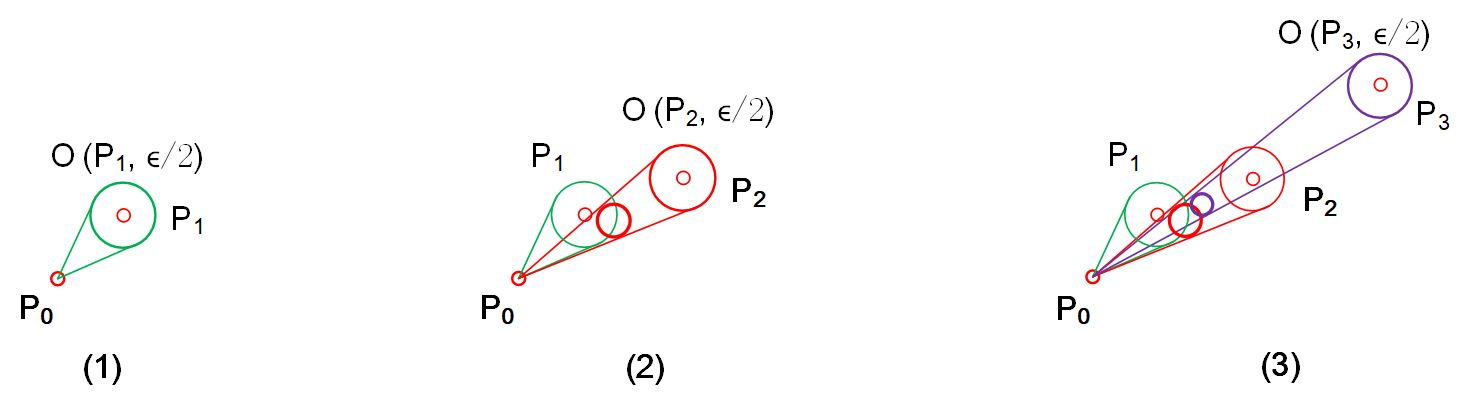
\includegraphics[scale=0.66]{Figures/Fig-Conest.jpg}
	\vspace{-1ex}
	\caption{\small A running example of the \cised algorithm. The points and the oblique circular cones are projected on an x-y space. }%The trajectory $\dddot{\mathcal{T}}[P_0, \ldots, P_{10}]$ is compressed into four line segments.
	\vspace{-2ex}
	\label{fig:exm-conest}
\end{figure}
%%%%%%%%%%%%%%%%

\begin{example}
	\label{exm-alg-conest}
	Figure~\ref{fig:exm-conest} shows a running example of algorithm \cised($\frac{\epsilon}{2}$) for compressing the trajectory \trajec{T} in Figure~\ref{fig:dp}.
	For convenience, we project the points and the oblique circular cones on an x-y space.
	%	
	(1) After initialization, the \cised algorithm reads point $P_1$ and builds a narrow \emph{oblique circular cone}~\cone{(P_0, \mathcal{O}(P_{1}, \epsilon/2))}, taking $P_0$ as its apex and \circle{(P_1, \epsilon/2)} as its base (green dash). The \emph{circular cone} is projected on the plane $P.t-P_1.t=0$, and the inscribe regular polygon $\mathcal{R}_1$ of the projection circle is returned. As $\mathcal{R}^*$ is empty, $\mathcal{R}^*$ is set to $\mathcal{R}_1$.
	%	
	(2) The algorithm reads $P_2$ and builds \cone{(P_0, \mathcal{O}(P_{2}, \epsilon/2))} (red dash). The \emph{circular cone} is also projected on the plane $P.t-P_1.t=0$ and the inscribe regular polygon $\mathcal{R}_2$ of the projection circle is returned. As $\mathcal{R}^*=\mathcal{R}_1$ is not empty, $\mathcal{R}^*$ is set to the intersection of $\mathcal{R}_2$ and $\mathcal{R}^*$, which is $\mathcal{R}_1 \bigsqcap \mathcal{R}_2 \ne \emptyset$.
	%	
	(3) For point $P_3$, the algorithm runs the same routine as $P_2$ until the intersection of $\mathcal{R}_3$ and $\mathcal{R}^*$ is $\emptyset$. Thus, a line segment $\vv{P_0P_2}$ is generated, and the process of a new line segment is started, taking $P_2$ as the new start point and $P.t-P_3.t=0$ as the new projection plane.
	%	
	(4) At last, the algorithm outputs four continuous line segments, \ie $\{\vv{P_0P_2}$, $\vv{P_2P_4}$, $\vv{P_4P_{7}}$, $\vv{P_7P_{10}}\}$. %\eop
\end{example} 	


\begin{figure}[tb!]
	\centering
	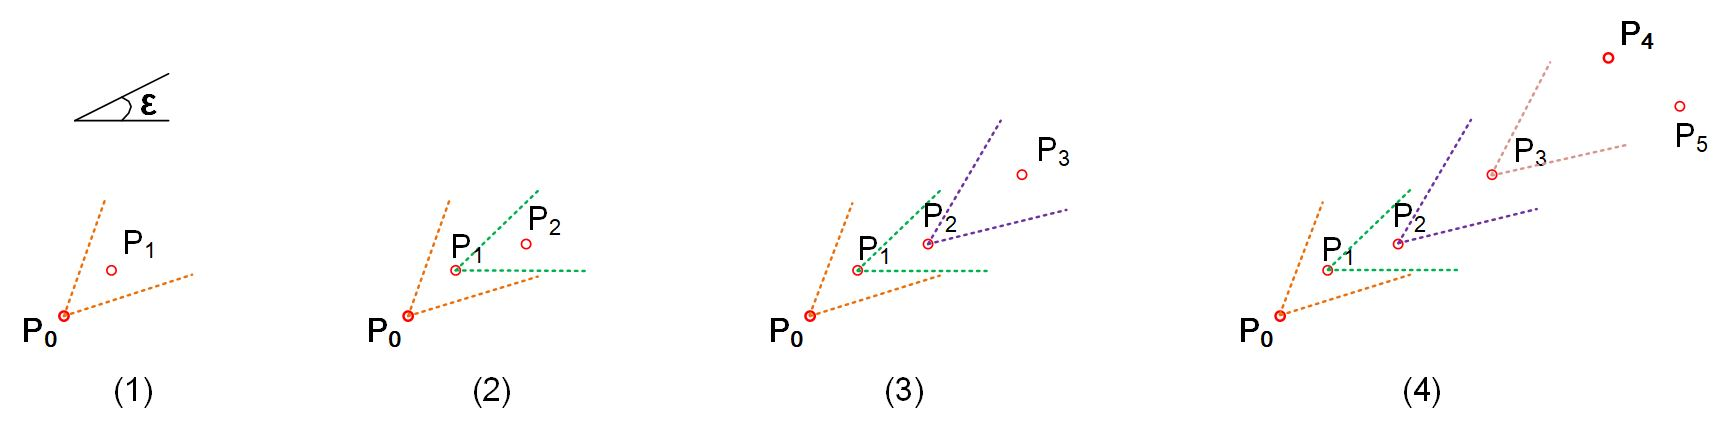
\includegraphics[scale=0.66]{Figures/Fig-interval.jpg}
	\vspace{-1ex}
	\caption{\small The trajectory $\dddot{\mathcal{T}}$ is compressed by the interval algorithm using \dad to two line segments.}
	\vspace{-1ex}
	\label{fig:interval}
\end{figure}




\subsubsection{Algorithms \intersec \cite{Long:Direction} and \interval \cite{Ke:Interval} Using \dad}
It designs a \emph{direction range} for each line segment connecting two neighboring points, then checks the common intersection of those \emph{direction ranges} as a way similar to the \emph{sector intersection} approach \cite{Williams:Longest, Sklansky:Cone, Dunham:Cone, Zhao:Sleeve}.

Given a direction line segment $\mathcal{L}$ and an angle $\epsilon$, the \emph{direction range} denoted by $range(\mathcal{L}.\theta, \epsilon)$ is $[\mathcal{L}.\theta-\epsilon, \mathcal{L}.\theta+\epsilon]$, which denotes the varying range of a directed line segment originated from the origin when it is rotated anti-clockwise from $\theta_1$ to $\theta_2$  \cite{Long:Direction}.
%
The {common intersection} of \emph{direction ranges} of directed line segments $\{\vv{P_sP_{s+1}}, \vv{P_{s+1}P_{s+2}}, ..., \vv{P_{s+k-1}P_{s+k}}\}$ \wrt $\epsilon$ is $\bigsqcap_{i=1}^{k}Range(\vv{P_{s+i-1} P_{s+i}}.\theta, \epsilon)$.
%denoted by $ComSub(\{\vv{P_sP_{s+1}}, \vv{P_{s+1}P_{s+2}}, ..., \vv{P_{s+k-1}P_{s+k}}\}, \epsilon)$,

Algorithm \intersec\cite{Long:Direction} uses a half range, and shows that if the {common intersection} $\bigsqcap_{i=1}^{k}range(\vv{P_{s+i-1} P_{s+i}}.\theta, \epsilon/2)$ is not empty, then the angular between $\vv{P_{s+i-1}P_{s+i}}$ and $\vv{P_sP_{s+k}}$ for all $i\in [1, k]$ is not larger than $\epsilon$.
%
Recently, algorithm \interval \cite{Ke:Interval} extends \intersec from half to full ranges, by showing that if the {common intersection} $\bigsqcap_{i=1}^{k}range(\vv{P_{s+i-1} P_{s+i}}.\theta, \epsilon)$ is not empty and $\vv{P_sP_{s+k}}.\theta$ falls in the {common intersection}, then the angular between $\vv{P_{s+i-1}P_{s+i}}$ and $\vv{P_sP_{s+k}}$ for all $i\in [1, k]$ is not larger than $\epsilon$.


\begin{example}
	\label{exm-alg-interval}
	Figure~\ref{fig:interval} is a running example of the \emph{interval} method taking as input the same trajectory $\dddot{\mathcal{T}}[P_0, \ldots, P_{10}]$. At the beginning, $P_0$ is the first start point, and points $P_1$, $P_2$, $P_3$, etc., each has a \emph{direction range} $Range(\vv{P_0P_1}, \epsilon)$, $Range(\vv{P_1P_2}, \epsilon)$, $Range(\vv{P_2P_3}, \epsilon)$, etc., respectively.
	%
	Because $\bigsqcap_{i=1}^{4}Range(\vv{P_{0+i-1}P_{0+i}}, \epsilon) \ne \phi$ and $\vv{P_0P_{4}}.\theta$ falls in the \emph{common subinterval}, and $\bigsqcap_{i=1}^{5}Range(\vv{P_{0+i-1}P_{0+i}}, \epsilon) = \phi$, $\vv{P_0P_4}$ is output and $P_4$ becomes the start point of the next section.
	At last, the algorithm outputs two continuous line segments $\vv{P_0P_4}$ and $\vv{P_4P_{10}}$.
\end{example}





